
\SetKwFunction{FDPTimelines}{DPTimelines}
\begin{figure}[htp]
\begin{minipage}[t]{0.49\textwidth}
    \centering
    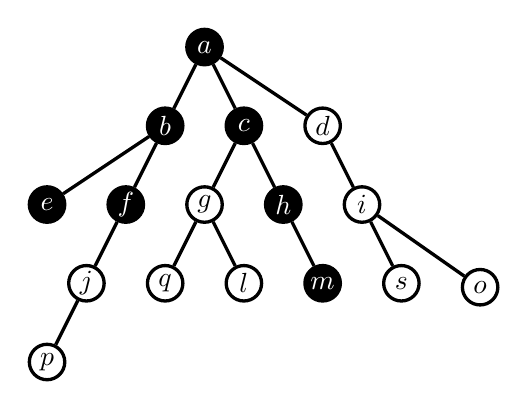
\begin{tikzpicture}[every path/.style={very thick}]

    \node[text=white, circle, draw, minimum size=0.45cm, inner sep=0pt, fill=black] (1) at (0,0) {$a$};

    \node[text=white, circle, draw, minimum size=0.45cm, inner sep=0pt, fill=black] (2) at (-0.5,-1) {$b$};

    \node[text=white, circle, draw, minimum size=0.45cm, inner sep=0pt, fill=black] (3) at (0.5,-1) {$c$};

    \node[circle, draw, minimum size=0.45cm, inner sep=0pt] (4) at (1.5,-1) {$d$};

    \draw[] (1) to (2);
    \draw[] (1) to (3);
    \draw[] (1) to (4);
    

    \node[text=white, circle, draw, minimum size=0.45cm, inner sep=0pt, fill=black] (5) at (-2,-2) {$e$};

    \node[text=white, circle, draw, minimum size=0.45cm, inner sep=0pt, fill=black] (6) at (-1,-2) {$f$};

    \node[circle, draw, minimum size=0.45cm, inner sep=0pt] (7) at (0,-2) {$g$};

    \node[text=white, circle, draw, minimum size=0.45cm, inner sep=0pt, fill=black] (8) at (1,-2) {$h$};

    \node[circle, draw, minimum size=0.45cm, inner sep=0pt] (9) at (2,-2) {$i$};

    \draw[] (2) to (5);
    \draw[] (2) to (6);

    \draw[] (3) to (7);
    \draw[] (3) to (8);

    \draw[] (4) to (9);

    \node[circle, draw, minimum size=0.45cm, inner sep=0pt] (10) at (-1.5,-3) {$j$};

    \node[circle, draw, minimum size=0.45cm, inner sep=0pt] (11) at (-0.5,-3) {$q$};

    \node[circle, draw, minimum size=0.45cm, inner sep=0pt] (12) at (0.5,-3) {$l$};

    \node[text=white, circle, draw, minimum size=0.45cm, inner sep=0pt, fill=black] (13) at (1.5,-3) {$m$};

    \node[circle, draw, minimum size=0.45cm, inner sep=0pt] (14) at (2.5,-3) {$s$};

    \node[circle, draw, minimum size=0.45cm, inner sep=0pt] (15) at (3.5,-3.05) {$o$};

    \draw[] (6) to (10);

    \draw[] (7) to (11);
    \draw[] (7) to (12);

    \draw[] (8) to (13);

    \draw[] (9) to (14);
    \draw[] (9) to (15);

    \node[circle, draw, minimum size=0.45cm, inner sep=0pt] (16) at (-2,-4) {$p$};


    \draw[] (10) to (16);

    
    \end{tikzpicture}
    \caption[Example tree $T$]{}\label{box_dt_input}
\end{minipage}
\begin{minipage}[t]{0.49\textwidth}
    \centering
    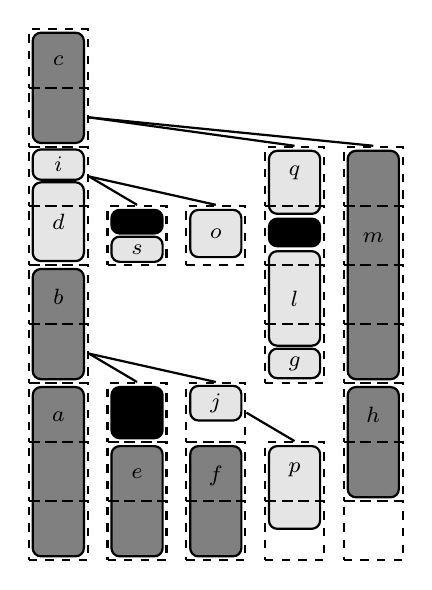
\begin{tikzpicture}[ every path/.style={thick}]
        \footnotesize
    \node[draw, 
        rounded corners=3pt, 
        minimum width=0.65cm, 
        minimum height=1.4cm, 
        align=center, fill=gray
        ] (A) at (0,-0.375) {\raisebox{0.7cm}{$c$}};

    \node[draw, 
        rounded corners=3pt, 
        minimum width=0.65cm, 
        minimum height=0.3cm, 
        align=center, fill=gray!20
        ] (A) at (0,-1.35) {$i$};
    
    \node[draw, 
        rounded corners=3pt, 
        minimum width=0.65cm, 
        minimum height=1.0cm, 
        align=center, fill=gray!20
        ] (A) at (0,-2.075) {$d$};

    \node[draw, 
        rounded corners=3pt, 
        minimum width=0.65cm, 
        minimum height=1.4cm, 
        align=center, fill=gray
        ] (A) at (0,-3.375) {\raisebox{0.7cm}{$b$}};

    \node[draw, 
        rounded corners=3pt, 
        minimum width=0.65cm, 
        minimum height=2.15cm, 
        align=center, fill=gray
        ] (A) at (0,-5.25) {\raisebox{1.4cm}{$a$}};

    \node[circle,  draw, dashed, rectangle, minimum size=0.75cm, inner sep=0pt] (11) at (0,0) {};

    \node[circle, draw, dashed, rectangle, minimum size=0.75cm, inner sep=0pt] (12) at (0,-0.75) {};

    \node[circle, draw, dashed, rectangle, minimum size=0.75cm, inner sep=0pt] (13) at (0,-1.5) {};

    \node[circle, draw, dashed, rectangle, minimum size=0.75cm, inner sep=0pt] (14) at (0,-2.25) {};

    \node[circle, draw, dashed, rectangle, minimum size=0.75cm, inner sep=0pt] (15) at (0,-3) {};

    \node[circle, draw, dashed, rectangle, minimum size=0.75cm, inner sep=0pt] (16) at (0,-3.75) {};

    \node[circle, draw, dashed, rectangle, minimum size=0.75cm, inner sep=0pt] (17) at (0,-4.5) {};

    \node[circle, draw, dashed, rectangle, minimum size=0.75cm, inner sep=0pt] (18) at (0,-5.25) {};
    
    \node[circle, draw, dashed, rectangle, minimum size=0.75cm, inner sep=0pt] (19) at (0,-6) {};

    \node[draw, 
        rounded corners=3pt, 
        minimum width=0.65cm, 
        minimum height=0.3cm, 
        align=center, fill=black
        ] (A) at (1,-2.075) {};
    
    \node[draw, 
        rounded corners=3pt, 
        minimum width=0.65cm, 
        minimum height=0.3cm, 
        align=center, fill=gray!20
        ] (A) at (1,-2.425) {$s$};
    
    \node[circle, draw, dashed, rectangle, minimum size=0.75cm, inner sep=0pt] (24) at (1,-2.25) {};

    \draw[] (13.east) to (24.north);

    \node[draw, 
        rounded corners=3pt, 
        minimum width=0.65cm, 
        minimum height=0.65cm, 
        align=center, fill=black
        ] (A) at (1,-4.5) {};

    \node[draw, 
        rounded corners=3pt, 
        minimum width=0.65cm, 
        minimum height=1.4cm, 
        align=center, fill=gray
        ] (A) at (1,-5.625) {\raisebox{0.7cm}{$e$}};

    \node[circle, draw, dashed, rectangle, minimum size=0.75cm, inner sep=0pt] (27) at (1,-4.5) {};

    \node[circle, draw, dashed, rectangle, minimum size=0.75cm, inner sep=0pt] (28) at (1,-5.25) {};
    
    \node[circle, draw, dashed, rectangle, minimum size=0.75cm, inner sep=0pt] (29) at (1,-6) {};

    \draw[] (16.east) to (27.north);

    \node[draw, 
        rounded corners=3pt, 
        minimum width=0.65cm, 
        minimum height=0.6cm, 
        align=center, fill=gray!20
        ] (A) at (2,-2.225) {$o$};
    
    \node[circle, draw, dashed, rectangle, minimum size=0.75cm, inner sep=0pt] (34) at (2,-2.25) {};

    \draw[] (13.east) to (34.north);

    \node[draw, 
        rounded corners=3pt, 
        minimum width=0.65cm, 
        minimum height=0.3cm, 
        align=center, fill=gray!20
        ] (A) at (2,-4.38) {$j$};
    
    \node[draw, 
        rounded corners=3pt, 
        minimum width=0.65cm, 
        minimum height=1.4cm, 
        align=center, fill=gray
        ] (A) at (2,-5.625) {\raisebox{0.7cm}{$f$}};

    \node[circle, draw, dashed, rectangle, minimum size=0.75cm, inner sep=0pt] (37) at (2,-4.5) {};

    \node[circle, draw, dashed, rectangle, minimum size=0.75cm, inner sep=0pt] (38) at (2,-5.25) {};
    
    \node[circle, draw, dashed, rectangle, minimum size=0.75cm, inner sep=0pt] (39) at (2,-6) {};

    \draw[] (16.east) to (37.north);

    
    \node[draw, 
        rounded corners=3pt, 
        minimum width=0.65cm, 
        minimum height=0.8cm, 
        align=center, fill=gray!20
        ] (A) at (3,-1.575) {\raisebox{0.3cm}{$q$}};

    \node[draw, 
        rounded corners=3pt, 
        minimum width=0.65cm, 
        minimum height=0.35cm, 
        align=center, fill=black
        ] (A) at (3,-2.212) {};


    \node[draw, 
        rounded corners=3pt, 
        minimum width=0.65cm, 
        minimum height=1.2cm, 
        align=center, fill=gray!20
        ] (A) at (3,-3.05) {$l$};

    \node[draw, 
        rounded corners=3pt, 
        minimum width=0.65cm, 
        minimum height=0.3cm, 
        align=center, fill=gray!20
        ] (A) at (3,-3.875) {$g$};

    \node[circle, draw, dashed, rectangle, minimum size=0.75cm, inner sep=0pt] (43) at (3,-1.5) {};

    \node[circle, draw, dashed, rectangle, minimum size=0.75cm, inner sep=0pt] (44) at (3,-2.25) {};
    
    \node[circle, draw, dashed, rectangle, minimum size=0.75cm, inner sep=0pt] (45) at (3,-3) {};

    \node[circle, draw, dashed, rectangle, minimum size=0.75cm, inner sep=0pt] (46) at (3,-3.75) {};

    \draw[] (12.east) to (43.north);

    \node[draw, 
        rounded corners=3pt, 
        minimum width=0.65cm, 
        minimum height=1.05cm, 
        align=center, fill=gray!20
        ] (A) at (3,-5.45) {\raisebox{0.5cm}{$p$}};

    \node[circle, draw, dashed, rectangle, minimum size=0.75cm, inner sep=0pt] (48) at (3,-5.25) {};
    
    \node[circle, draw, dashed, rectangle, minimum size=0.75cm, inner sep=0pt] (49) at (3,-6) {};

    \draw[] (37.east) to (48.north);

    \node[draw, 
        rounded corners=3pt, 
        minimum width=0.65cm, 
        minimum height=2.9cm, 
        align=center, fill=gray
        ] (A) at (4,-2.625) {\raisebox{0.7cm}{$m$}};

    \node[draw, 
        rounded corners=3pt, 
        minimum width=0.65cm, 
        minimum height=1.4cm, 
        align=center, fill=gray
        ] (A) at (4,-4.875) {\raisebox{0.7cm}{$h$}};

    \node[circle, draw, dashed, rectangle, minimum size=0.75cm, inner sep=0pt] (53) at (4,-1.5) {};

    \node[circle, draw, dashed, rectangle, minimum size=0.75cm, inner sep=0pt] (54) at (4,-2.25) {};

    \node[circle, draw, dashed, rectangle, minimum size=0.75cm, inner sep=0pt] (55) at (4,-3) {};

    \node[circle, draw, dashed, rectangle, minimum size=0.75cm, inner sep=0pt] (56) at (4,-3.75) {};

    \node[circle, draw, dashed, rectangle, minimum size=0.75cm, inner sep=0pt] (57) at (4,-4.5) {};

    \node[circle, draw, dashed, rectangle, minimum size=0.75cm, inner sep=0pt] (58) at (4,-5.25) {};
    
    \node[circle, draw, dashed, rectangle, minimum size=0.75cm, inner sep=0pt] (59) at (4,-6) {};

    \draw[] (12.east) to (53.north);
    
    \end{tikzpicture}
    \caption[Example boxed decision tree $D$]{}\label{box_dt}
\end{minipage}

\caption[Structure of a boxed decision tree]{Structure of a boxed decision tree. Figure \ref{box_dt_input} shows example input tree $T$, black vertices are heavy and white vertices are white. Figure \ref{box_dt} shows example boxed decision tree $D$ for $T$, dark gray queries are heavy, light gray queries are light, and black spaces represent additional load of boxes.}\label{box_dt_figure}
\end{figure}